\documentclass[a4paper, 12pt]{article}
\usepackage[utf8]{inputenc}
\DeclareUnicodeCharacter{00B2}{\ensuremath{{}^2}}
\usepackage{listings}
\usepackage{graphicx}
\title{Obligatorisk innlevering 1}
\author{Sivert M. Skarning}
\date{Mai 2019}
\begin{document}
\maketitle
\section{Oppgave 1}
\paragraph{Oppgavebeskrivelse}
Implementer konvolusjon på egen hånd. Implementasjonen skal være generell slik at den kan anvendes på alle bilder og filtere. Det er greit å begrense implementasjonen til å fungere på gråskalabilder, men det er ikke påkrevd. Implementasjonen skal støtte minst to ulike former for utvidelse/padding. Rapporten skal inneholde dokumentasjon for at implementasjonen fungerer.
\subsection{Dokumentasjon}
Vedlagt ligger et script kalt convolution.py. Koden utfører konvolusjon på bilde man legger ved som argument. Scriptet gir brukeren mulighet til å velge filterstørrelse of hvilke verdier filteret har. Brukeren har også mulighet til å velge mellom to forskjellige paddingmuligheter, zeropadding og reflectionpadding. Zeropadding er implementert med egenprogramert funksjon navngitt zero-pad.
Reflectionpad blir implmentert med pakken numpy og er navngitt np.pad. Begge funksjonene fungerer hvor zero-pad gir svart ramme rundt generert bild og reflectionpad gir utvidelse av bilde. Uten padding ville bruk av flere filtere etterhvert krympe bilde betydlig.
Selve implmentasjonen er inneffektivt implementert og i praksis ville man brukt en annen algoritme for å gjøre en konvolusjon. O-notasjonen for min implementsjon vil være: $$O(n² * m²)$$

\lstinputlisting[caption=Convolve function, language=Python, breaklines=true]{convolve.py}

\subsection{Resultat}
For å teste konvolveringsalgoritmen har jeg valgt å påføre tre typer filtere på lena.png.

\begin{figure}[h]
  \centering
  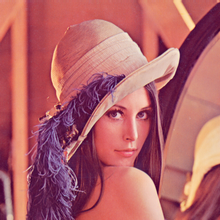
\includegraphics[width=0.5\textwidth]{images/lena}
  \caption{Bilde av Lena, et vanlig eksempel i bildebehandling}
  \label{fig:lena}
\end{figure}

\begin{itemize}
   \item Laplacian sharpening
   \item Mean blure
   \item Gaussian blure
\end{itemize}

\begin{figure}[h]
  \centering
  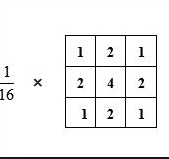
\includegraphics[width=0.5\textwidth]{images/gaussian-filter}
  \caption{Gaussian filter}
  \label{fig:gaussian-filter}
\end{figure}

\begin{figure}[h]
  \centering
  
\includegraphics[width=0.5\textwidth]{images/gaussian-blurred-lena}
  \caption{Lena konvolvert med filteret på Figur \ref{fig:gaussian-filter}}
  \label{fig:gaussian-blurred-lena}
\end{figure}

\paragraph{Gaussain blure} Konvolverings algoritmen fungerte bra. Her med egenimplementert zeropadding. Hadde først problemer med dårlig kontrast på bildet. Reskalerte intensiteten før bilde ble lagret, og fikk dermed et godt resultat som sett i figur \ref{fig:gaussian-blurred-lena}.

\paragraph{Mean blure}
Forskjellen mellom gaussian blure og mena blure for dette eksempelet er minimal. Ved større filtere ville man kunne se større forskjell. Man trenger vanligvis å kjøre gjennom et mean filter 4 ganger for å få den samme effekten som ved et gaussisk filter. Implementasjonen av konvolverings programmet er uheldig, da man heller skulle lagd det som et set med funksjoner man kunne kalle i steder for å lage det som et skript med bilde som argument. På denne måten kunne man ha testet større filtere lettere.

\begin{figure}[h]
  \centering
  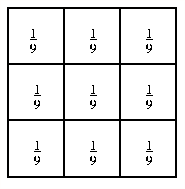
\includegraphics[width=0.5\textwidth]{images/mean-filter}
  \caption{Mean filter}
  \label{fig:mean-blure}
\end{figure}

\begin{figure}[h]
  \centering
  
\includegraphics[width=0.5\textwidth]{images/mean-blure-lena}
  \caption{Lena konvolvert med filteret på Figur \ref{fig:mean-blure}}
  \label{fig:mean-blurred-lena}
\end{figure}

\paragraph{Laplacian sharpening}
Laplacian filteret fremhever raske endringer i et bilde. På denne måten blir bilde skarpere, fordi vi kan se kantene på bilde bedere. Man vil se dette på figur \ref{fig:lena-laplacian} i forhold til figur \ref{fig:lena}.

\begin{figure}[h]
  \centering
  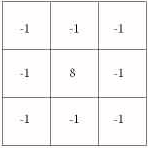
\includegraphics[width=0.5\textwidth]{images/laplacian-filter}
  \caption{Laplacian filter}
  \label{fig:laplacian-filter}
\end{figure}

\begin{figure}[h]
  \centering
  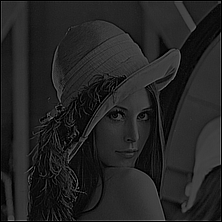
\includegraphics[width=0.5\textwidth]{images/laplacian-lena}
  \caption{Lena konvolvert med filteret på Figur \ref{fig:laplacian-filter}}
  \label{fig:lena-laplacian}
\end{figure}
\end{document}